
%% bare_jrnl.tex
%% V1.4b
%% 2015/08/26
%% by Michael Shell
%% see http://www.michaelshell.org/
%% for current contact information.
%%
%% This is a skeleton file demonstrating the use of IEEEtran.cls
%% (requires IEEEtran.cls version 1.8b or later) with an IEEE
%% journal paper.
%%
%% Support sites:
%% http://www.michaelshell.org/tex/ieeetran/
%% http://www.ctan.org/pkg/ieeetran
%% and
%% http://www.ieee.org/

%%*************************************************************************
%% Legal Notice:
%% This code is offered as-is without any warranty either expressed or
%% implied; without even the implied warranty of MERCHANTABILITY or
%% FITNESS FOR A PARTICULAR PURPOSE! 
%% User assumes all risk.
%% In no event shall the IEEE or any contributor to this code be liable for
%% any damages or losses, including, but not limited to, incidental,
%% consequential, or any other damages, resulting from the use or misuse
%% of any information contained here.
%%
%% All comments are the opinions of their respective authors and are not
%% necessarily endorsed by the IEEE.
%%
%% This work is distributed under the LaTeX Project Public License (LPPL)
%% ( http://www.latex-project.org/ ) version 1.3, and may be freely used,
%% distributed and modified. A copy of the LPPL, version 1.3, is included
%% in the base LaTeX documentation of all distributions of LaTeX released
%% 2003/12/01 or later.
%% Retain all contribution notices and credits.
%% ** Modified files should be clearly indicated as such, including  **
%% ** renaming them and changing author support contact information. **
%%*************************************************************************


% *** Authors should verify (and, if needed, correct) their LaTeX system  ***
% *** with the testflow diagnostic prior to trusting their LaTeX platform ***
% *** with production work. The IEEE's font choices and paper sizes can   ***
% *** trigger bugs that do not appear when using other class files.       ***                          ***
% The testflow support page is at:
% http://www.michaelshell.org/tex/testflow/



\documentclass[journal]{IEEEtran}
%
% If IEEEtran.cls has not been installed into the LaTeX system files,
% manually specify the path to it like:
% \documentclass[journal]{../sty/IEEEtran}





% Some very useful LaTeX packages include:
% (uncomment the ones you want to load)


% *** MISC UTILITY PACKAGES ***
%
%\usepackage{ifpdf}
% Heiko Oberdiek's ifpdf.sty is very useful if you need conditional
% compilation based on whether the output is pdf or dvi.
% usage:
% \ifpdf
%   % pdf code
% \else
%   % dvi code
% \fi
% The latest version of ifpdf.sty can be obtained from:
% http://www.ctan.org/pkg/ifpdf
% Also, note that IEEEtran.cls V1.7 and later provides a builtin
% \ifCLASSINFOpdf conditional that works the same way.
% When switching from latex to pdflatex and vice-versa, the compiler may
% have to be run twice to clear warning/error messages.






% *** CITATION PACKAGES ***
%
%\usepackage{cite}
% cite.sty was written by Donald Arseneau
% V1.6 and later of IEEEtran pre-defines the format of the cite.sty package
% \cite{} output to follow that of the IEEE. Loading the cite package will
% result in citation numbers being automatically sorted and properly
% "compressed/ranged". e.g., [1], [9], [2], [7], [5], [6] without using
% cite.sty will become [1], [2], [5]--[7], [9] using cite.sty. cite.sty's
% \cite will automatically add leading space, if needed. Use cite.sty's
% noadjust option (cite.sty V3.8 and later) if you want to turn this off
% such as if a citation ever needs to be enclosed in parenthesis.
% cite.sty is already installed on most LaTeX systems. Be sure and use
% version 5.0 (2009-03-20) and later if using hyperref.sty.
% The latest version can be obtained at:
% http://www.ctan.org/pkg/cite
% The documentation is contained in the cite.sty file itself.






% *** GRAPHICS RELATED PACKAGES ***
%
\ifCLASSINFOpdf
   \usepackage[pdftex]{graphicx}
  % declare the path(s) where your graphic files are
  % \graphicspath{{../pdf/}{../jpeg/}}
  % and their extensions so you won't have to specify these with
  % every instance of \includegraphics
  % \DeclareGraphicsExtensions{.pdf,.jpeg,.png}
\else
  % or other class option (dvipsone, dvipdf, if not using dvips). graphicx
  % will default to the driver specified in the system graphics.cfg if no
  % driver is specified.
  % \usepackage[dvips]{graphicx}
  % declare the path(s) where your graphic files are
  % \graphicspath{{../eps/}}
  % and their extensions so you won't have to specify these with
  % every instance of \includegraphics
  % \DeclareGraphicsExtensions{.eps}
\fi
% graphicx was written by David Carlisle and Sebastian Rahtz. It is
% required if you want graphics, photos, etc. graphicx.sty is already
% installed on most LaTeX systems. The latest version and documentation
% can be obtained at: 
% http://www.ctan.org/pkg/graphicx
% Another good source of documentation is "Using Imported Graphics in
% LaTeX2e" by Keith Reckdahl which can be found at:
% http://www.ctan.org/pkg/epslatex
%
% latex, and pdflatex in dvi mode, support graphics in encapsulated
% postscript (.eps) format. pdflatex in pdf mode supports graphics
% in .pdf, .jpeg, .png and .mps (metapost) formats. Users should ensure
% that all non-photo figures use a vector format (.eps, .pdf, .mps) and
% not a bitmapped formats (.jpeg, .png). The IEEE frowns on bitmapped formats
% which can result in "jaggedy"/blurry rendering of lines and letters as
% well as large increases in file sizes.
%
% You can find documentation about the pdfTeX application at:
% http://www.tug.org/applications/pdftex





% *** MATH PACKAGES ***
%
%\usepackage{amsmath}
% A popular package from the American Mathematical Society that provides
% many useful and powerful commands for dealing with mathematics.
%
% Note that the amsmath package sets \interdisplaylinepenalty to 10000
% thus preventing page breaks from occurring within multiline equations. Use:
%\interdisplaylinepenalty=2500
% after loading amsmath to restore such page breaks as IEEEtran.cls normally
% does. amsmath.sty is already installed on most LaTeX systems. The latest
% version and documentation can be obtained at:
% http://www.ctan.org/pkg/amsmath





% *** SPECIALIZED LIST PACKAGES ***
%
%\usepackage{algorithmic}
% algorithmic.sty was written by Peter Williams and Rogerio Brito.
% This package provides an algorithmic environment fo describing algorithms.
% You can use the algorithmic environment in-text or within a figure
% environment to provide for a floating algorithm. Do NOT use the algorithm
% floating environment provided by algorithm.sty (by the same authors) or
% algorithm2e.sty (by Christophe Fiorio) as the IEEE does not use dedicated
% algorithm float types and packages that provide these will not provide
% correct IEEE style captions. The latest version and documentation of
% algorithmic.sty can be obtained at:
% http://www.ctan.org/pkg/algorithms
% Also of interest may be the (relatively newer and more customizable)
% algorithmicx.sty package by Szasz Janos:
% http://www.ctan.org/pkg/algorithmicx




% *** ALIGNMENT PACKAGES ***
%
%\usepackage{array}
% Frank Mittelbach's and David Carlisle's array.sty patches and improves
% the standard LaTeX2e array and tabular environments to provide better
% appearance and additional user controls. As the default LaTeX2e table
% generation code is lacking to the point of almost being broken with
% respect to the quality of the end results, all users are strongly
% advised to use an enhanced (at the very least that provided by array.sty)
% set of table tools. array.sty is already installed on most systems. The
% latest version and documentation can be obtained at:
% http://www.ctan.org/pkg/array


% IEEEtran contains the IEEEeqnarray family of commands that can be used to
% generate multiline equations as well as matrices, tables, etc., of high
% quality.




% *** SUBFIGURE PACKAGES ***
%\ifCLASSOPTIONcompsoc
%  \usepackage[caption=false,font=normalsize,labelfont=sf,textfont=sf]{subfig}
%\else
%  \usepackage[caption=false,font=footnotesize]{subfig}
%\fi
% subfig.sty, written by Steven Douglas Cochran, is the modern replacement
% for subfigure.sty, the latter of which is no longer maintained and is
% incompatible with some LaTeX packages including fixltx2e. However,
% subfig.sty requires and automatically loads Axel Sommerfeldt's caption.sty
% which will override IEEEtran.cls' handling of captions and this will result
% in non-IEEE style figure/table captions. To prevent this problem, be sure
% and invoke subfig.sty's "caption=false" package option (available since
% subfig.sty version 1.3, 2005/06/28) as this is will preserve IEEEtran.cls
% handling of captions.
% Note that the Computer Society format requires a larger sans serif font
% than the serif footnote size font used in traditional IEEE formatting
% and thus the need to invoke different subfig.sty package options depending
% on whether compsoc mode has been enabled.
%
% The latest version and documentation of subfig.sty can be obtained at:
% http://www.ctan.org/pkg/subfig




% *** FLOAT PACKAGES ***
%
%\usepackage{fixltx2e}
% fixltx2e, the successor to the earlier fix2col.sty, was written by
% Frank Mittelbach and David Carlisle. This package corrects a few problems
% in the LaTeX2e kernel, the most notable of which is that in current
% LaTeX2e releases, the ordering of single and double column floats is not
% guaranteed to be preserved. Thus, an unpatched LaTeX2e can allow a
% single column figure to be placed prior to an earlier double column
% figure.
% Be aware that LaTeX2e kernels dated 2015 and later have fixltx2e.sty's
% corrections already built into the system in which case a warning will
% be issued if an attempt is made to load fixltx2e.sty as it is no longer
% needed.
% The latest version and documentation can be found at:
% http://www.ctan.org/pkg/fixltx2e


%\usepackage{stfloats}
% stfloats.sty was written by Sigitas Tolusis. This package gives LaTeX2e
% the ability to do double column floats at the bottom of the page as well
% as the top. (e.g., "\begin{figure*}[!b]" is not normally possible in
% LaTeX2e). It also provides a command:
%\fnbelowfloat
% to enable the placement of footnotes below bottom floats (the standard
% LaTeX2e kernel puts them above bottom floats). This is an invasive package
% which rewrites many portions of the LaTeX2e float routines. It may not work
% with other packages that modify the LaTeX2e float routines. The latest
% version and documentation can be obtained at:
% http://www.ctan.org/pkg/stfloats
% Do not use the stfloats baselinefloat ability as the IEEE does not allow
% \baselineskip to stretch. Authors submitting work to the IEEE should note
% that the IEEE rarely uses double column equations and that authors should try
% to avoid such use. Do not be tempted to use the cuted.sty or midfloat.sty
% packages (also by Sigitas Tolusis) as the IEEE does not format its papers in
% such ways.
% Do not attempt to use stfloats with fixltx2e as they are incompatible.
% Instead, use Morten Hogholm'a dblfloatfix which combines the features
% of both fixltx2e and stfloats:
%
% \usepackage{dblfloatfix}
% The latest version can be found at:
% http://www.ctan.org/pkg/dblfloatfix




%\ifCLASSOPTIONcaptionsoff
%  \usepackage[nomarkers]{endfloat}
% \let\MYoriglatexcaption\caption
% \renewcommand{\caption}[2][\relax]{\MYoriglatexcaption[#2]{#2}}
%\fi
% endfloat.sty was written by James Darrell McCauley, Jeff Goldberg and 
% Axel Sommerfeldt. This package may be useful when used in conjunction with 
% IEEEtran.cls'  captionsoff option. Some IEEE journals/societies require that
% submissions have lists of figures/tables at the end of the paper and that
% figures/tables without any captions are placed on a page by themselves at
% the end of the document. If needed, the draftcls IEEEtran class option or
% \CLASSINPUTbaselinestretch interface can be used to increase the line
% spacing as well. Be sure and use the nomarkers option of endfloat to
% prevent endfloat from "marking" where the figures would have been placed
% in the text. The two hack lines of code above are a slight modification of
% that suggested by in the endfloat docs (section 8.4.1) to ensure that
% the full captions always appear in the list of figures/tables - even if
% the user used the short optional argument of \caption[]{}.
% IEEE papers do not typically make use of \caption[]'s optional argument,
% so this should not be an issue. A similar trick can be used to disable
% captions of packages such as subfig.sty that lack options to turn off
% the subcaptions:
% For subfig.sty:
% \let\MYorigsubfloat\subfloat
% \renewcommand{\subfloat}[2][\relax]{\MYorigsubfloat[]{#2}}
% However, the above trick will not work if both optional arguments of
% the \subfloat command are used. Furthermore, there needs to be a
% description of each subfigure *somewhere* and endfloat does not add
% subfigure captions to its list of figures. Thus, the best approach is to
% avoid the use of subfigure captions (many IEEE journals avoid them anyway)
% and instead reference/explain all the subfigures within the main caption.
% The latest version of endfloat.sty and its documentation can obtained at:
% http://www.ctan.org/pkg/endfloat
%
% The IEEEtran \ifCLASSOPTIONcaptionsoff conditional can also be used
% later in the document, say, to conditionally put the References on a 
% page by themselves.




% *** PDF, URL AND HYPERLINK PACKAGES ***
%
\usepackage{url}
% url.sty was written by Donald Arseneau. It provides better support for
% handling and breaking URLs. url.sty is already installed on most LaTeX
% systems. The latest version and documentation can be obtained at:
% http://www.ctan.org/pkg/url
% Basically, \url{my_url_here}.




% *** Do not adjust lengths that control margins, column widths, etc. ***
% *** Do not use packages that alter fonts (such as pslatex).         ***
% There should be no need to do such things with IEEEtran.cls V1.6 and later.
% (Unless specifically asked to do so by the journal or conference you plan
% to submit to, of course. )


% correct bad hyphenation here
\hyphenation{op-tical net-works semi-conduc-tor}


\begin{document}
%
% paper title
% Titles are generally capitalized except for words such as a, an, and, as,
% at, but, by, for, in, nor, of, on, or, the, to and up, which are usually
% not capitalized unless they are the first or last word of the title.
% Linebreaks \\ can be used within to get better formatting as desired.
% Do not put math or special symbols in the title.
\title{Reader Authentication Protocol for\\EPCglobal C1G2 CRFID Tags}
%
%
% author names and IEEE memberships
% note positions of commas and nonbreaking spaces ( ~ ) LaTeX will not break
% a structure at a ~ so this keeps an author's name from being broken across
% two lines.
% use \thanks{} to gain access to the first footnote area
% a separate \thanks must be used for each paragraph as LaTeX2e's \thanks
% was not built to handle multiple paragraphs
%

\author{Jonathan~Blieschke}
%\author{Michael~Shell,~\IEEEmembership{Member,~IEEE,}
%        John~Doe,~\IEEEmembership{Fellow,~OSA,}
%        and~Jane~Doe,~\IEEEmembership{Life~Fellow,~IEEE}% <-this % stops a space
%\thanks{M. Shell was with the Department
%of Electrical and Computer Engineering, Georgia Institute of Technology, Atlanta,
%GA, 30332 USA e-mail: (see http://www.michaelshell.org/contact.html).}% <-this % stops %a space
%\thanks{J. Doe and J. Doe are with Anonymous University.}% <-this % stops a space
%\thanks{Manuscript received April 19, 2005; revised August 26, 2015.}}

% note the % following the last \IEEEmembership and also \thanks - 
% these prevent an unwanted space from occurring between the last author name
% and the end of the author line. i.e., if you had this:
% 
% \author{....lastname \thanks{...} \thanks{...} }
%                     ^------------^------------^----Do not want these spaces!
%
% a space would be appended to the last name and could cause every name on that
% line to be shifted left slightly. This is one of those "LaTeX things". For
% instance, "\textbf{A} \textbf{B}" will typeset as "A B" not "AB". To get
% "AB" then you have to do: "\textbf{A}\textbf{B}"
% \thanks is no different in this regard, so shield the last } of each \thanks
% that ends a line with a % and do not let a space in before the next \thanks.
% Spaces after \IEEEmembership other than the last one are OK (and needed) as
% you are supposed to have spaces between the names. For what it is worth,
% this is a minor point as most people would not even notice if the said evil
% space somehow managed to creep in.



% The paper headers
%\markboth{Journal of \LaTeX\ Class Files,~Vol.~14, No.~8, August~2015}%
%{Shell \MakeLowercase{\textit{et al.}}: Bare Demo of IEEEtran.cls for IEEE Journals}
% The only time the second header will appear is for the odd numbered pages
% after the title page when using the twoside option.
% 
% *** Note that you probably will NOT want to include the author's ***
% *** name in the headers of peer review papers.                   ***
% You can use \ifCLASSOPTIONpeerreview for conditional compilation here if
% you desire.




% If you want to put a publisher's ID mark on the page you can do it like
% this:
%\IEEEpubid{0000--0000/00\$00.00~\copyright~2015 IEEE}
% Remember, if you use this you must call \IEEEpubidadjcol in the second
% column for its text to clear the IEEEpubid mark.



% use for special paper notices
%\IEEEspecialpapernotice{(Invited Paper)}




% make the title area
\maketitle

% As a general rule, do not put math, special symbols or citations
% in the abstract or keywords.
\begin{abstract}
    With Computational RFID tags being put to use in wireless sensor networks, protocols are being developed which allow a sensor's firmware to be updated wirelessly in deeply-embedded applications.
    So far, little work has been done to enable secure updates, such that only authorized readers can install firmware onto tags.
    We have implemented a reader authentication protocol for the WISP5 CRFID tag.
    While the protocol we have implemented is not completely secure, we have proposed modifications and extensions which improve the security while still allowing it to be implemented on top of the WISP5's relatively limited firmware.
    Continued work in this area could bring about a cryptographically secure wireless firmware update protocol.
\end{abstract}

% Note that keywords are not normally used for peerreview papers.
%\begin{IEEEkeywords}
%IEEE, IEEEtran, journal, \LaTeX, paper, template.
%\end{IEEEkeywords}






% For peer review papers, you can put extra information on the cover
% page as needed:
% \ifCLASSOPTIONpeerreview
% \begin{center} \bfseries EDICS Category: 3-BBND \end{center}
% \fi
%
% For peerreview papers, this IEEEtran command inserts a page break and
% creates the second title. It will be ignored for other modes.
\IEEEpeerreviewmaketitle



\section{Introduction}
% The very first letter is a 2 line initial drop letter followed
% by the rest of the first word in caps.
% 
% form to use if the first word consists of a single letter:
% \IEEEPARstart{A}{demo} file is ....
% 
% form to use if you need the single drop letter followed by
% normal text (unknown if ever used by the IEEE):
% \IEEEPARstart{A}{}demo file is ....
% 
% Some journals put the first two words in caps:
% \IEEEPARstart{T}{his demo} file is ....
% 
% Here we have the typical use of a "T" for an initial drop letter
% and "HIS" in caps to complete the first word.
%\IEEEPARstart{T}{his} demo file is intended to serve as a ``starter file''
%for IEEE journal papers produced under \LaTeX\ using
%IEEEtran.cls version 1.8b and later.
% You must have at least 2 lines in the paragraph with the drop letter
% (should never be an issue)
%I wish you the best of success.

%\hfill mds
 
%\hfill August 26, 2015

% %%% REPORT PLAN %%%
% Tag Security -> Assessment of WISP5 -> Firmware Insufficient by Itself
% Potentially Vulnerable Applications -> OTA Firmware Update (R2 & Wisent)
% No OTA Firmware Update Protocols Currently Require Reader Verification
% Propose Protocol for Reader Verification + OTA Update Compatability
% > Introduction
% > Previous Work
%  - EPCglobal C1G2 Protocol v2.0
%  - OTA Firmware Updates
%  - CRFID Verification / Authentication Protocols
% > Protocol
%  - Description
%  - Issues \& Modifications
% > Future Work
%  - ...
% > Conclusion
% 

\IEEEPARstart{T}{his} project began with an investigation into the security measures available on a Wireless Identification and Sensing Platform revision 5 (WISP5) CRFID tag.\cite{wisp}
Recognising that RFID tags are becoming more commonplace for inventory purposes, and the potential uses for CRFID devices in wireless sensor networks, we originally hoped to find and exploit a vulnerability in the WISP5 firmware, and possibly implement a fix.
We began with an investigation into the EPCglobal protocol version 1.2,\cite{epc12} which we believed to be current at the time when the WISP5 firmware was developed.
We examined the protocol specification, looking for ways in which a reader could interact with a tag which might cause the tag to behave unexpectedly, if care was not taken when writing the firmware.
\\\\
Initially, we identified a number of commands with variable lengths, as these could have been vulnerable to a buffer overflow.
We also noticed that commands such as \textit{BlockWrite}, if not bounds-checked, could possibly be used to read or write areas of memory which are not supposed to be accessible.
The usefulness of such a vulnerability would depend on the layout of the tag's memory, and the range of accessible locations.
Shortly after we began looking through the WISP5 code, we were quite disappointed.
No variable-length commands were correctly implemented, and the parameters read from \textit{Read}, \textit{Write} and \textit{BlockWrite} commands were stored in a globally-accessible structure in the tag's memory rather than being handled in accordance with the protocol specification.
When each of the commands were completed, they would call `hook' functions, which are intended to be implemented by other developers to extend the WISP5's behaviour.
The write hook, for instance, could be used to decide whether the data sent by the reader should be stored in the tag's non-volatile memory, and if so, where.
Since the default implementations of these hooks is a single no-op, we realised that any vulnerabilities we found would need to be in applications built on top of the firmware.
\\\\
While searching for academic papers which had implemented useful applications on the WISP5, two papers on wireless firmware updates caught our attention. \cite{r2,wisent}
Both of these papers acknowledged that they lacked any form of protection, allowing attackers to plant their own firmware on the tag, and recommended that this be a focus of future work.
So, shifting our focus slightly away from exploiting vulnerabilities, we turned our attention to the other part of our goal and attempted to secure these wireless update protocols.
We decided against recommending the \textit{Access} command described in the EPCglobal version 1.2 specification, as it is trivial to steal the tag's access password by eavesdropping on its exchange with the reader.

\section{Previous Work}
    \subsection{Over-the-Air Firmware Update}
        The R$^2$\cite{r2} and Wisent\cite{wisent} papers both present similar mechanisms for transmitting new firmware to a tag, utilising the \textit{Write} command's MemBank field to differentiate between different reprogramming stages.
        Both protocols use a MemBank of $00_2$ to begin the reprogramming process, $01_2$ to write a piece of the new firmware, and $10_2$ to end the reprogramming process, executing the new firmware.
        Performing regular writes to the tag's data memory is done with a MemBank of $11_2$.
        \\\\
        Both protocols also outline a bootloader which allows multiple `applications' to be installed on a tag, and for different applications to be selected and run.
        Both papers cite Bootie,\cite{bootie} an earlier proposal for a CRFID bootloader which aimed to achieve the same goal.
        One noticeable difference from Bootie is that both of these papers use the execution command to select which application is run, allowing a reader to execute one arbitrarily with a single command.
        \\\\
        The two most significant security risks on tags which implement these protocols are the installation and execution of firmware by an unauthorised reader.
        In order to effectively secure this protocol, a reader must be prevented from beginning the reprogramming process and from executing an installed application unless it has been authenticated.
        Security measures which are implemented at the EPC protocol level - such as the \textit{Access} command - would be suitable, but are not implemented on the WISP5.
    \subsection{EPCglobal Protocol Version 2}
        In 2015, EPCglobal released an update to the C1G2 protocol.\cite{epc20}
        Significant extensions were included as optional features, many of which directly addressed the security concerns in the older protocol.
        Several new commands were added, including\textit{Challenge}, \textit{Authenticate}, \textit{SecureComm}, \textit{AuthComm}, \textit{KeyUpdate} and \textit{TagPrivilege}.
        \\\\
        The \textit{Authenticate} command is an alternative to \textit{Access}, which was present in the previous protocol version.
        Like \textit{Access}, \textit{Authenticate} causes a tag to transition from the open state into the secured state.
        Unlike \textit{Access}, it uses one of the cryptographic suites present on the tag to verify the reader, the tag, or both.
        The cryptographic suites available on a particular tag are defined by the manufacturer, and a parameter passed to the \textit{Authenticate} command specifies which suite is to be used.
        Some suites may require multiple commands in order to authenticate successfully.
        \textit{Challenge} is used to instruct multiple tags to prepare for a subsequent authentication.
        As with \textit{Authenticate}, one of its parameters specifies which cryptographic suite should be used.
        \\\\
        A tag may contain a number of cryptographic keys, with each key having an individually assigned list of privileges.
        When a reader authenticates with a particular key, the commands which it may send to a tag depend upon the privileges associated with the key it used.
        The \textit{KeyUpdate} command is used to modify keys, if the key used to authenticate has appropriate privileges.
        The \textit{TagPrivilege} command is used to modify the privileges granted to keys, if the key used to authenticate already has appropriate privileges.
        \textit{AuthComm} and \textit{SecureComm} are used to securely encapsulate other commands, in a manner specified by the cryptographic suite.
        \\\\
        These protocol extensions outline a general security framework for CRFID tags and their data, including the possibility of role-based authorization.
        Implementing a firmware update protocol on a tag which supports mutual cryptographic authentication would eliminate the existing security concerns.
        Since the framework outlined in this updated specification is an industry standard, it provides a solid foundation for designing an authentication protocol suited to a more specific purpose.
\section{Reader Authentication Protocol}
    \subsection{Description}
        Our first idea for securing the wireless update protocols was to improve the security of the EPCglobal 1.2 access procedure.
        The reader begins by sending a \textit{ReqRN} command to the tag, which backscatters a random number.
        The reader uses this number to cover-code the 16 most-significant bits of the 32-bit access password, which it sends back to the tag.
        The reader then issues another \textit{ReqRN}, and the process repeats for the 16 least-significant bits of the access password.
        If both halves of the password are received correctly, the tag transitions into the secure state.
        The most obvious problem with this procedure is that an eavesdropper could easily steal the password.
        By overhearing both random numbers and both cover-coded halves of the password, the attacker has enough information to uncover the entire password, compromising the security of the tag.
        This issue could be solved relatively simply, by having the tag encrypt the random number before sending it.
        Thus, when the tag receives a correctly cover-coded password, it can be certain that the reader also shares its encryption key, and the password cannot be stolen by eavesdropping.
        While this does appear to fix the problem, any tag which implements this solution exactly as stated is no longer compliant with the EPCglobal specification.
        Implementing this solution on the WISP5 would also be challenging, since significant amounts of time-sensitive assembly code would need to be modified.
        An easier solution would be to implement a similar system as an application on top of the WISP5 firmware.
        Some care would need to be taken to ensure that the implementation remains compatible with the wireless update protocols, but small adjustments could be made to either protocol in the interests of improving their security.
        \begin{figure*}[!t]
            \centering
            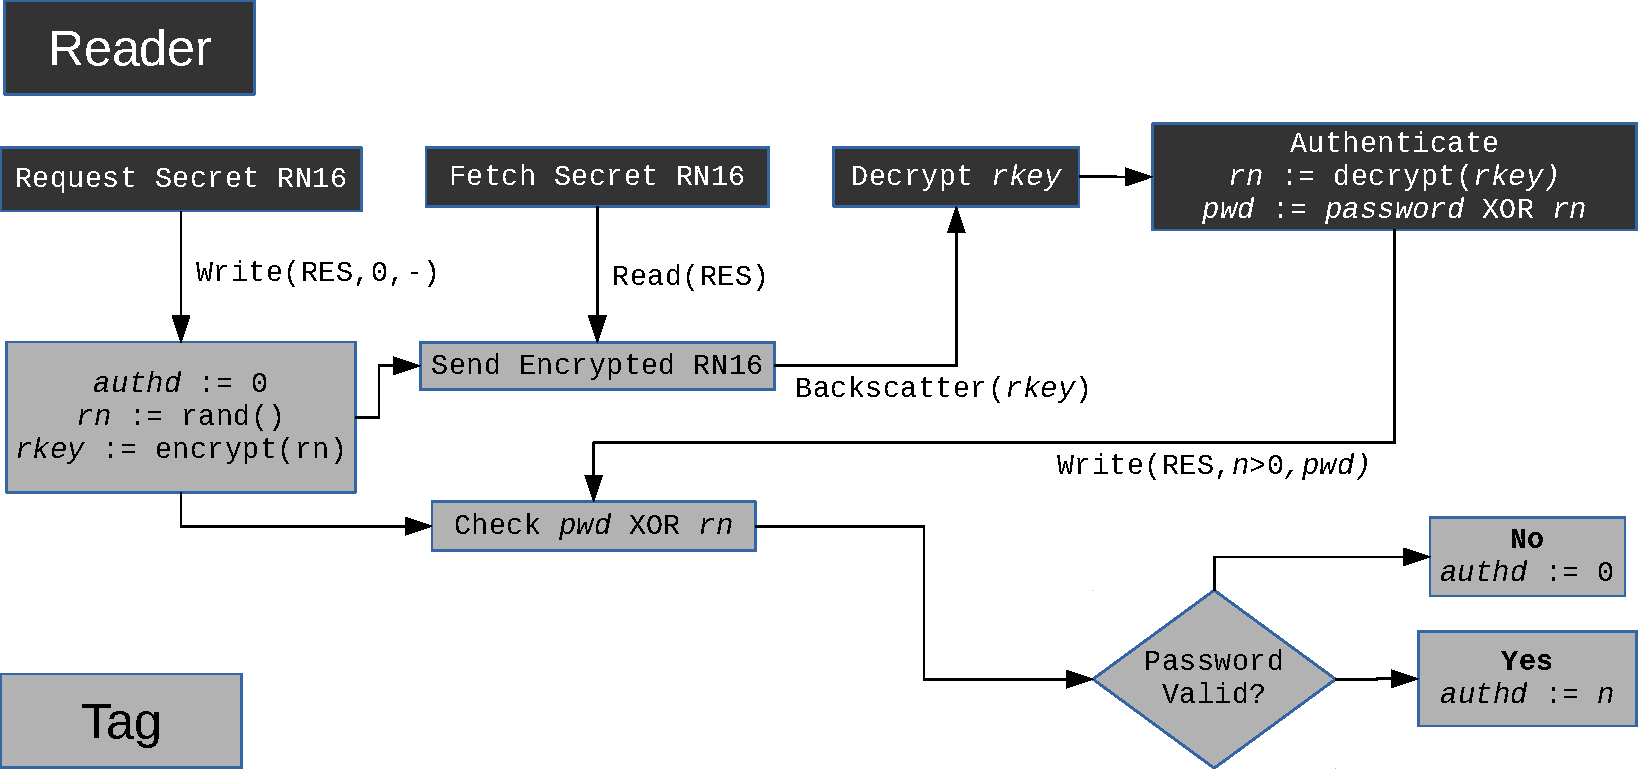
\includegraphics[width=0.75\textwidth]{images/CRFID-Auth-Process.pdf}
            \caption{Flowchart of the Authentication Protocol}
            \label{proto-diag}
        \end{figure*}
        \\\\
        To begin our implementation of an access procedure, we need to be able to encode the \textit{ReqRN} and \textit{Access} commands within other commands, such as \textit{Read} or \textit{Write}.
        First, the tag must be instructed to generate and encrypt a random number.
        Borrowing an idea from the wireless update protocols, we set aside a particular \textit{Write} command to initiate the authentication procedure.
        Since the WISP5 does not implement password protection, use of the reserved memory bank ($00_2$) for access-specific commands seems appropriate.
        Performing a \textit{Write} to the reserved memory bank with WordPtr set to zero will cause the tag to generate a new random number, encrypt it, and store the encrypted value in the memory bank at WordPtr = 4.
        This requires some slight modification of the WISP5's default layout, as its reserved bank usually resides in volatile memory.
        However, modifying the pointer in the relevant global structure resolves this problem.
        The EPCglobal specification does not specifically prohibit the inclusion of other data in the reserved memory bank, so this protocol remains compatible.
        The data sent to the tag via this write command is ignored.
        At the next stage, the reader must read the encrypted random number out of the tag's memory.
        Issuing a \textit{Read} command to the reserved bank with WordPtr = 4 will retrieve the data stored in the memory bank.
        The random number itself will only be 16 bits long, but more data may need to be read depending on which cipher was used.
        Our implementation used AES, a 128-bit block cipher, requiring that we read the entire ciphertext from the tag.
        The \textit{Read} command allows up to 255 words (4,080 bits) to be read from a single command, so this is easily achieved.
        The reader will decrypt the received random number, and use it to cover-code a 16-bit password, much like the one used in the EPCglobal access procedure.
        The reader will then send this cover-coded password back to the tag.
        It should be sent via a \textit{Write} command to the tag's reserved bank, with WordPtr $>$ 0.
        The tag will check that the received password is correct, thus verifying that the reader it is communicating with has both its password and its cryptographic key.
        Thus, the reader is considered authenticated until it instructs the tag to generate a new random number.
        Figure \ref{proto-diag} illustrates the protocol we implemented.
        \\\\
        A reader's authentication status only affects its ability to write to the tag's memory, and not its ability to read like the EPCglobal access procedure.
        Since this is sufficient to protect the wireless update protocols from malicious firmware, this protocol is still sufficient to address the most significant concerns identified in their respective papers.
        There are several reasons for this limitation, mostly related to simplifying the implementation.
        Writing data to the tag's memory is handled by hooks, which the tag's firmware calls after the command is processed, but the read hook is not called until the data has already been transmitted to the reader.
        Checking the tag's authentication status before responding to a read would require the modification of time-sensitive assembly code.
        The tag would also need to allow the encrypted random number to be read, but nothing else, which complicates the necessary checks.
    \subsection{Possible Extensions}
        We considered some possible extensions to this protocol, such as having 'sessions' which expire after a specified number of writes.
        The value of WordPtr on the second \textit{Write} would be used to set a counter, which is decremented whenever a write is performed.
        Written data is only stored in the tag memory if the counter is greater than zero.
        When the tag is instructed to generate a new random number, it resets the counter to zero.
        Expiring sessions may be useful for quickly writing a fixed amount of data to a tag, as it removes the need for an additional command to de-authenticate when the writes are complete.
        However, in a streaming application like a Wisent data transfer, a limit of 255 successive writes may simply be an inconvenience.
        The other possible protocol extension was inspired by the support for multiple keys and encryption methods in the updated EPCglobal protocol.
        The data sent by the first \textit{Write} command to initialise the authentication procedure could be used to specify which key and/or encryption method to use, if more than one is supported.
        This could be extended further by only allowing some keys to write new applications onto the tag, while others are allowed to execute existing applications.
        Alternatively, this data field could be used to encode commands for a more complex authentication protocol.
        An example of such a protocol will be described later.
    \subsection{Implementation}
        Our implementation used AES, a 128-bit block cipher, recommended by a colleague as one of the better algorithms implemented by the BLOC project.\cite{bloc,altbloc}
        The 16-bit random number we generated was stored in the first two bytes of the encrypted block.
        The rest of the block was unspecified values, often zeroed out or populated with the value FF3F$_{16}$.
        We hard-coded the encryption key into the tag's firmware.
        We implemented the entire tag-side protocol within the write hook, deciding what to do primarily based on the MemBank field and an authentication flag outside of the tag's accessible memory.
        We also ensured that the unencrypted random number was not accessible via \textit{Read} command.
        We implemented the session-counter extension, where each authenticated write would decrement the authentication counter.
        Unfortunately, our implementation mistakenly placed the reserved memory bank, unencrypted random number and authentication counter in volatile memory, preventing it from working when the tag is not connected to a debugger.
        We did not realise this error until we no longer had enough time to fix it.
    \subsection{Problems \& Possible Solutions}
        While a high-level description of this protocol seems relatively secure, there are still a number of problems.
        First, due to the limited computational resources available on a passive CRFID tag like the WISP5, having the tag calculate a random number is not ideal.
        The WISP5 specifically uses a lookup table, which makes the `random' numbers it generates relatively predictable.
        The second problem is the length of the tag's password.
        The 32-bit password used by the EPCglobal access procedure has been criticised\cite{smartcard} for its vulnerability to a brute-force attack.
        The shorter 16-bit password used in this protocol is significantly easier to guess, which would also allow an attacker to bypass decrypting the random number.
        These two vulnerabilities are significant, but by no means irreparable.
        However, both solutions would benefit from a \textit{BlockWrite} implementation which adheres to the EPCglobal specification.
        The WISP5 is designed to work with a reader which does not issue the \textit{BlockWrite} command correctly.
        Instead of writing the block of data in a single command, the reader issues a series of \textit{BlockWrites}, each one writing only a single word of data, making it effectively equivalent to an ordinary \textit{Write}.
        These proposed solutions will initially assume a correctly-implemented \textit{BlockWrite}, and then a more complex solution will follow for the WISP5.
        \\\\
        To initiate the authentication procedure, the reader writes an encrypted random number into the tag's reserved memory bank, at WordPtr = 0.
        For ciphers like AES, with a block size larger than 16 bits, a \textit{BlockWrite} is necessary to send the entire ciphertext in a single command.
        The tag resets its authentication state, decrypts the random number, and prepares to receive a cover-coded password.
        The encrypted random number is not saved to the reserved bank, but the decrypted number is stored in memory which cannot be accessed with a \textit{Read} command.
        The reader then writes a cover-coded password to the tag's reserved memory bank at WordPtr $>$ 0.
        The tag checks the password, and the reader is successfully authenticated.
        This protocol allows both major problems to be solved at once.
        Because the reader generates the random number, not the tag, much more computational power is available, so the number will be harder to guess than the existing solution.
        The use of \textit{BlockWrite} also allows much longer random numbers and passwords to be used, significantly reducing the likelihood that an attacker can simply use brute-force to obtain access to the tag.
        The random number and password could both utilise the cipher's full block size, rather than being restricted to the first two bytes.
        \\\\
        \begin{table}[!t]
            \renewcommand{\arraystretch}{1.3}
            \caption{Example of Additional Commands Embedded in the Data Field}
            \label{data-cmd}
            \centering
            \begin{tabular}{|c|c|c|c|}
                \hline
                 & RFU & Sending & Data\\
                \hline
                Bits & 6 & 2 & 8\\
                \hline
                Use & - & \parbox[t]{1.2in}{$00_2$: Reset Authentication \\$01_2$: Random Number \\$10_2$: Password \\$11_2$: Set Expiration} & Data\\
                \hline
            \end{tabular}
        \end{table}
        To implement an improved protocol on the WISP5, modifications must be made to remove the need for a \textit{BlockWrite} command.
        We propose that these modifications could make use of the data field in the first command of our existing protocol.
        If the 16-bit data field of this command is used to encode other protocol-specific commands, such as beginning the transfer of a multiple-byte ciphertext.
        Table \ref{data-cmd} illustrates a simple example of the behaviour which could be embedded in the data field.
        When a \textit{Write} is received to the reserved memory bank with WordPtr = 0, the data field is not written to the tag's memory but is parsed as a protocol command.
        The first six bits are currently unused.
        The next two bits encode the command which the tag should parse.
        $00_2$ indicates that the tag should reset its current authentication status.
        $01_2$ indicates that the next series of writes to the reserved memory bank will be the encrypted random number.
        Each write in the series will use the WordPtr field to indicate the order in which they should be stored.
        $10_2$ indicates that the next series of writes to the reserved memory bank will be the cover-coded password.
        Writes will behave the same as for transmitting the random number.
        $11_2$ indicates that the tag's expiration counter should be set to the value stored in the data field.
        If the data field contains a zero, the reader's authentication will not expire until it is reset.
        While the implementation of this protocol would be challenging, it would allow tags to authenticate a reader before saving data to their memory banks.
        In order to allow compatibility with R$^2$ or Wisent, this protocol may require further modification, but this should provide a sold foundation for future work in this area.
\section{Future Work}
    Despite the progress that we have made in this direction, more work yet needs to be done before wireless firmware update protocols like R$^2$ or Wisent can benefit from this reader authentication protocol.
    Conflicts in functionality between their reprogramming commands and the first command from this protocol need to be identified and resolved, then the combined secure protocol needs to be implemented.
    Further extensions to the combined protocol could allow for the implementation of a system which brings functionality similar to version 2.0 of the EPCglobal specification onto devices which only support an older version.
    Further analysis could also be done on which cryptographic cipher is most suitable for this particular application, as our implementation was based on a cursory reading of the BLOC project analysis paper.
\section{Conclusion}
    We have implemented a reader authentication protocol for the WISP5 CRFID tag.
    While the protocol we have implemented is not completely secure, we have proposed modifications and extensions which improve the security while still allowing it to be implemented on the WISP5's relatively limited firmware.
    Continued work in this area could bring about a cryptographically secure wireless firmware update protocol.
%\subsection{Subsection Heading Here}
%Subsection text here.

% needed in second column of first page if using \IEEEpubid
%\IEEEpubidadjcol

%\subsubsection{Subsubsection Heading Here}
%Subsubsection text here.


% An example of a floating figure using the graphicx package.
% Note that \label must occur AFTER (or within) \caption.
% For figures, \caption should occur after the \includegraphics.
% Note that IEEEtran v1.7 and later has special internal code that
% is designed to preserve the operation of \label within \caption
% even when the captionsoff option is in effect. However, because
% of issues like this, it may be the safest practice to put all your
% \label just after \caption rather than within \caption{}.
%
% Reminder: the "draftcls" or "draftclsnofoot", not "draft", class
% option should be used if it is desired that the figures are to be
% displayed while in draft mode.
%
%\begin{figure}[!t]
%\centering
%\includegraphics[width=2.5in]{myfigure}
% where an .eps filename suffix will be assumed under latex, 
% and a .pdf suffix will be assumed for pdflatex; or what has been declared
% via \DeclareGraphicsExtensions.
%\caption{Simulation results for the network.}
%\label{fig_sim}
%\end{figure}

% Note that the IEEE typically puts floats only at the top, even when this
% results in a large percentage of a column being occupied by floats.


% An example of a double column floating figure using two subfigures.
% (The subfig.sty package must be loaded for this to work.)
% The subfigure \label commands are set within each subfloat command,
% and the \label for the overall figure must come after \caption.
% \hfil is used as a separator to get equal spacing.
% Watch out that the combined width of all the subfigures on a 
% line do not exceed the text width or a line break will occur.
%
%\begin{figure*}[!t]
%\centering
%\subfloat[Case I]{\includegraphics[width=2.5in]{box}%
%\label{fig_first_case}}
%\hfil
%\subfloat[Case II]{\includegraphics[width=2.5in]{box}%
%\label{fig_second_case}}
%\caption{Simulation results for the network.}
%\label{fig_sim}
%\end{figure*}
%
% Note that often IEEE papers with subfigures do not employ subfigure
% captions (using the optional argument to \subfloat[]), but instead will
% reference/describe all of them (a), (b), etc., within the main caption.
% Be aware that for subfig.sty to generate the (a), (b), etc., subfigure
% labels, the optional argument to \subfloat must be present. If a
% subcaption is not desired, just leave its contents blank,
% e.g., \subfloat[].


% An example of a floating table. Note that, for IEEE style tables, the
% \caption command should come BEFORE the table and, given that table
% captions serve much like titles, are usually capitalized except for words
% such as a, an, and, as, at, but, by, for, in, nor, of, on, or, the, to
% and up, which are usually not capitalized unless they are the first or
% last word of the caption. Table text will default to \footnotesize as
% the IEEE normally uses this smaller font for tables.
% The \label must come after \caption as always.
%
%\begin{table}[!t]
%% increase table row spacing, adjust to taste
%\renewcommand{\arraystretch}{1.3}
% if using array.sty, it might be a good idea to tweak the value of
% \extrarowheight as needed to properly center the text within the cells
%\caption{An Example of a Table}
%\label{table_example}
%\centering
%% Some packages, such as MDW tools, offer better commands for making tables
%% than the plain LaTeX2e tabular which is used here.
%\begin{tabular}{|c||c|}
%\hline
%One & Two\\
%\hline
%Three & Four\\
%\hline
%\end{tabular}
%\end{table}


% Note that the IEEE does not put floats in the very first column
% - or typically anywhere on the first page for that matter. Also,
% in-text middle ("here") positioning is typically not used, but it
% is allowed and encouraged for Computer Society conferences (but
% not Computer Society journals). Most IEEE journals/conferences use
% top floats exclusively. 
% Note that, LaTeX2e, unlike IEEE journals/conferences, places
% footnotes above bottom floats. This can be corrected via the
% \fnbelowfloat command of the stfloats package.




%\section{Conclusion}
%The conclusion goes here.





% if have a single appendix:
%\appendix[Proof of the Zonklar Equations]
% or
%\appendix  % for no appendix heading
% do not use \section anymore after \appendix, only \section*
% is possibly needed

% use appendices with more than one appendix
% then use \section to start each appendix
% you must declare a \section before using any
% \subsection or using \label (\appendices by itself
% starts a section numbered zero.)
%


\appendices
%\section{Proof of the First Zonklar Equation}
%Appendix one text goes here.

% you can choose not to have a title for an appendix
% if you want by leaving the argument blank
%\section{}
%Appendix two text goes here.


% use section* for acknowledgment
%\section*{Acknowledgment}


%The authors would like to thank...


% Can use something like this to put references on a page
% by themselves when using endfloat and the captionsoff option.
%\ifCLASSOPTIONcaptionsoff
%  \newpage
%\fi



% trigger a \newpage just before the given reference
% number - used to balance the columns on the last page
% adjust value as needed - may need to be readjusted if
% the document is modified later
%\IEEEtriggeratref{8}
% The "triggered" command can be changed if desired:
%\IEEEtriggercmd{\enlargethispage{-5in}}

% references section

% can use a bibliography generated by BibTeX as a .bbl file
% BibTeX documentation can be easily obtained at:
% http://mirror.ctan.org/biblio/bibtex/contrib/doc/
% The IEEEtran BibTeX style support page is at:
% http://www.michaelshell.org/tex/ieeetran/bibtex/
%\bibliographystyle{IEEEtran}
% argument is your BibTeX string definitions and bibliography database(s)
%\bibliography{IEEEabrv,../bib/paper}
%
% <OR> manually copy in the resultant .bbl file
% set second argument of \begin to the number of references
% (used to reserve space for the reference number labels box)
\begin{thebibliography}{1}

%\bibitem{IEEEhowto:kopka}
%H.~Kopka and P.~W. Daly, \emph{A Guide to \LaTeX}, 3rd~ed.\hskip 1em plus
%  0.5em minus 0.4em\relax Harlow, England: Addison-Wesley, 1999.

\bibitem{wisp} https://wisp5.wikispaces.com/WISP+Home

\bibitem{epc12} EPC\texttrademark Radio-Frequency Identity Protocols 
Class-1 Generation-2 UHF RFID
Protocol for Communications at 860 MHz - 960 MHz
Version 1.2.0
(2008)
http://www.gs1.org/sites/default/files/docs/epc/uhfc1g2\_1\_2\_0-standard-20080511.pdf

\bibitem{r2} D. Wu, M. J. Hussain, S. Li and L. Lu, "R2: Over-the-air reprogramming on computational RFIDs," 2016 IEEE International Conference on RFID (RFID), Orlando, FL, USA, 2016, pp. 1-8.
doi: 10.1109/RFID.2016.7488004

\bibitem{wisent} Tan, Jethro, et al. "Wisent: Robust Downstream Communication and Storage for Computational RFIDs." arXiv preprint arXiv:1512.04602 (2015).

\bibitem{bootie} Ransford, Benjamin. "A Rudimentary Bootloader for Computational RFIDs." University of Massachusetts Amherst, Tech. Rep. UM-CS-2010-061 (2010).

\bibitem{epc20} EPC\texttrademark Radio-Frequency Identity Protocols Generation-2 UHF RFID
Specification for RFID Air Interface
Protocol for Communications at 860 MHz - 960 MHz
Version 2.0.1 Ratified
(2015)
http://www.gs1.org/sites/default/files/docs/epc/Gen2\_Protocol\_Standard.pdf

\bibitem{bloc} Mickaël Cazorla, Kevin Marquet, and Marine Minier. Survey and benchmark of lightweight block ciphers for wireless sensor networks. IACR Cryptology ePrint Archive, 2013:295, 2013. http://eprint.iacr.org/2013/295.pdf.
\bibitem{altbloc} Mickaël Cazorla, Kevin Marquet, and Marine Minier. Survey and benchmark of lightweight block ciphers for wireless sensor networks. In Pierangela Samarati, editor, SECRYPT 2013 - Proceedings of the 10th International Conference on Security and Cryptography, Reykjavík, Iceland, 29-31 July, 2013, pages 543-548. SciTePress, 2013.

\bibitem{smartcard} Contactless Smart Cards vs EPC Gen 2 RFID Tags: Frequently Asked Questions
http://www.smartcardalliance.org/publications-epc-gen2-faq/

\end{thebibliography}

% biography section
% 
% If you have an EPS/PDF photo (graphicx package needed) extra braces are
% needed around the contents of the optional argument to biography to prevent
% the LaTeX parser from getting confused when it sees the complicated
% \includegraphics command within an optional argument. (You could create
% your own custom macro containing the \includegraphics command to make things
% simpler here.)
%\begin{IEEEbiography}[{\includegraphics[width=1in,height=1.25in,clip,keepaspectratio]{mshell}}]{Michael Shell}
% or if you just want to reserve a space for a photo:

%\begin{IEEEbiography}{Michael Shell}
%Biography text here.
%\end{IEEEbiography}

% if you will not have a photo at all:
%\begin{IEEEbiographynophoto}{John Doe}
%Biography text here.
%\end{IEEEbiographynophoto}

% insert where needed to balance the two columns on the last page with
% biographies
%\newpage

%\begin{IEEEbiographynophoto}{Jane Doe}
%Biography text here.
%\end{IEEEbiographynophoto}

% You can push biographies down or up by placing
% a \vfill before or after them. The appropriate
% use of \vfill depends on what kind of text is
% on the last page and whether or not the columns
% are being equalized.

%\vfill

% Can be used to pull up biographies so that the bottom of the last one
% is flush with the other column.
%\enlargethispage{-5in}



% that's all folks
\end{document}


